%% ISANN vs ITERML comparison paper, draft v0, 2026-11-01 (Spain time).
%% Target: Combustion and Flame (Elsevier, elsarticle); alternative Energy and AI.
%% Base: ISANN article draft v1 (chemmanifold/isann/articulo/), ITERML roadmap and iteration reports.
%% \pending{} = ITERML iteration 2 result, due about 19:45 CET on 2026-11-01; fill from
%%   chemmanifold/iterml/iter2/eval_protocol_report.md, seeds_report.md, benchmark.md.
%% \todo{} = must be resolved before submission. Check every reference in refs.bib against the paper.
\documentclass[preprint,review,12pt]{elsarticle}

\usepackage[T1]{fontenc}
\usepackage{lmodern}
\usepackage{amsmath,amssymb}
\usepackage{graphicx}
\usepackage{booktabs}
\usepackage{siunitx}
\usepackage{lineno}
\usepackage{xcolor}
\usepackage{tikz}
\usetikzlibrary{positioning,arrows.meta,fit}
\usepackage[hidelinks]{hyperref}
\newcommand{\todo}[1]{\textcolor{red}{[TODO: #1]}}
\newcommand{\pending}[1]{\textcolor{orange!85!black}{[ITERML iter.~2: #1]}}
\sisetup{group-separator={\,},group-minimum-digits=4}
\linenumbers
\journal{Combustion and Flame}

\begin{document}
\begin{frontmatter}

\title{Where should the training data of a neural chemistry surrogate come from? Online learning from
direct integration versus physics-based re-exploration seeded by the simulation}

\author[a]{Javier \todo{surname}}
\author[a]{\todo{co-authors}}
\address[a]{\todo{affiliation}}

\begin{abstract}
Neural-network surrogates of finite-rate chemistry trained a priori on canonical reactors meet, in the
actual simulation, states they have not seen. Two ways of closing that gap with the help of the
simulation are compared on the same laminar methane/air burner, the same 18-species mechanism (GA18),
the same network architecture and the same evaluation protocol against direct integration (DI). In
\emph{ISANN} (in situ adaptive neural network), the running simulation trains its own surrogate: it starts
with DI, stores deduplicated (state, time step, DI result) pairs, fine-tunes a pre-trained network on
them and switches it in through an acceptance gate. In \emph{ITERML} (iterative machine learning), no
state of the simulation is ever a training pair: a run with the network collects the states where the
network is out of distribution or disagrees with sparse DI checks, these states are deduplicated and
used only as starting points of new Cantera reactor explorations (partially stirred reactors, relaxation,
ignition, cooling), and the network is retrained on physics data alone. Run without any DI fallback (the
only mode available in commercial solvers), the final ISANN network reached a mean flame-zone temperature
error of 2.1~K over 25--50~ms, and the first ITERML iteration 3.3~K (1.7~K at 50~ms), against 68.8~K for
the a priori network. Their start-up errors are mirror images: the ISANN network ignites the fuel jet
0.4~ms early, the ITERML network 0.6~ms late. ISANN gives better radicals and CO; ITERML keeps the training
data independent of the simulation, so the model remains a physics-based model of the mechanism, at the
cost of a slower growth of CO and heat release in the hot gas and a small loss on an offline benchmark of
canonical states. \pending{one sentence with the iteration-2 ignition time and flame error.}
\end{abstract}

\begin{keyword}
Chemistry acceleration \sep Neural network surrogate \sep Online learning \sep Active learning \sep
Thermochemical space exploration \sep Out-of-distribution detection
\end{keyword}
\end{frontmatter}

%% ===============================================================================================
\section{Introduction}
\label{sec:intro}

The integration of stiff finite-rate chemistry dominates the cost of many reacting-flow simulations.
Storage/retrieval methods such as in situ adaptive tabulation (ISAT)~\cite{pope1997isat} tabulate direct
integrations during the simulation itself; regression methods replace the integrator with a fitted map,
and artificial neural networks (ANN) have been used for this since the
1990s~\cite{christo1996ann,blasco1998ann}. The training data of such networks have come from the
simulation of a similar case~\cite{sen2010les}, from canonical laminar flames~\cite{ihme2009ann}, from
abstract problems that sample the composition space~\cite{franke2017rcce,ding2021hybrid,readshaw2021hybrid},
or have been used to fit neural ordinary differential equations~\cite{owoyele2022chemnode}.

Whatever the source, an a priori data set is a guess of the states the simulation will visit, and the
guess is never complete. Out-of-distribution (OOD) detectors with a DI fallback limit the damage, but a
fallback does not exist in every solver (a commercial code such as Ansys Fluent calls a user-defined
chemistry step that must return a result), and errors that build up over many steps inside the training
data are not detected by an OOD test. The simulation itself is the only reliable source of information on
the states it needs. The question this paper addresses is how that information should enter the
surrogate. Two answers are possible:
\begin{enumerate}
\item \emph{as labels}: the simulation integrates the states it visits with DI and the network is trained
  on those pairs. This is the ISAT idea transferred to a network; we call the scheme ISANN;
\item \emph{as locations}: the simulation only says \emph{where} the network fails, and the training data
  are generated by physics-based exploration started from those states. The data stay a model of the
  mechanism, not of the simulation; we call the loop ITERML.
\end{enumerate}
The first answer uses the most relevant data possible but ties the network to one simulation, and its
labels are produced by a solution that the network may already have biased. The second keeps the
training data independent of the CFD solution, which matters when the surrogate is to be reported as a
physics-based model, reused in another configuration, or validated against the same simulation it was
trained for, but it relies on the exploration to reproduce the relevant states from a seed.

We compare the two on the same burner, mechanism, network, exploration framework, OOD detector and
evaluation protocol, and report accuracy against DI during start-up and in the established flame,
species and heat release, generality on an offline benchmark of canonical states, and cost.
\todo{Literature on online/active learning of chemistry surrogates and adaptive sampling (e.g.\ active
learning of reaction manifolds, on-the-fly ANN tabulation, DeepFlame and similar frameworks); position
both schemes against it.}

%% ===============================================================================================
\section{Common elements}
\label{sec:common}

\subsection{Surrogate network}
The surrogate maps the composition at the start of a chemistry step to that at its end, at constant
pressure and enthalpy. Species mass fractions are Box--Cox transformed ($\lambda=0.1$) and standardised;
the context $c=(T,p,h,\log_{10}\Delta t)$ modulates a residual MLP through feature-wise linear modulation
(FiLM)~\cite{perez2018film} (three residual blocks, 192 hidden units, SiLU, layer normalisation, output
initialised to zero so that the untrained network is the identity). The temperature at the end of the
step follows from the predicted composition and the conserved enthalpy. Steps longer than the trained
range ($\Delta t_\mathrm{max}=\SI{4e-5}{s}$) are sub-stepped; cells below $T_\mathrm{freeze}=600$~K are
not advanced. The same C core is called by an OpenFOAM v2412 chemistry solver and by an Ansys Fluent
DEFINE\_CHEM\_STEP user-defined function.

\subsection{A priori exploration}
The a priori data come only from Cantera~\cite{cantera} calculations with the GA18 mechanism at the
burner's inlet conditions: 0D ignition and equilibrium relaxation, partially stirred reactors (PaSR),
steady and unsteady flamelets over a range of strain rates, vitiated mixing and heat-loss (cooling)
reactors (regimes 0--8). The pairs are integrated over a range of chemistry steps taken from the
histogram of the per-cell chemistry time step of the target solver. Successive revisions of this
exploration produced the networks ood1 to ood8; ISANN starts from ood7 and ITERML from ood8, the best
a priori network at the time each scheme was started (Section~\ref{sec:fair}).
\todo{Table of the a priori regimes and pair counts of ood7 and ood8.}

\subsection{Out-of-distribution detection and shadow checks}
Each exported model carries tables built from its own training data. A state is OOD if its temperature,
a species or the pressure leaves the trained range (globally or in its mixture-fraction band), if its
residual to a local principal-component manifold is too large, or if it is farther than $d_\mathrm{L}$
from the nearest of a set of training landmarks. \emph{Shadow checks} integrate a sample of cells with DI
from the same state as the network; the sample is stratified over bins of (temperature, mixture fraction,
inside/OOD) so that it covers all regions of the flame and not mostly the far field. A check fails if
$|T_\mathrm{ANN}-T_\mathrm{DI}|>\max(1\,\mathrm{K},\,0.3|T_\mathrm{DI}-T_0|)$ or if the analogous test on
OH (and in ITERML also H, O and CO; floor \num{5e-5}) fails.

\subsection{Deduplication}
Both schemes store states with the same two-level deduplication: a grid in $T$, $\sqrt{Z}$, the logarithm
of eight key species and $\log_{10}\Delta t$ with at most one state per box (reservoir sampling), and a
radius of novelty in the standardised coordinates of the OOD detector. On \num{902029} hot-cell DI states
of the burner the two levels reduce the states 93 times while every state stays within
$0.27\,d_\mathrm{L}$ of a kept one. ITERML adds a third level: a seed within the radius of any seed of an
earlier iteration is dropped.

\subsection{Test case}
\label{sec:case}
The burner is a laminar, non-premixed methane/air burner of a domestic cooking geometry, computed 2D
axisymmetric (5$^\circ$ wedge, 60k cells) with gravity. Pure CH$_4$ enters at 300~K through a central tube
($r<2.5$~mm, \num{6.7e-6}~kg/s, about 340~W), air through an annular co-flow and a slow outer co-flow; a pot
with convective walls ($h=15$~W\,m$^{-2}$K$^{-1}$, 323~K) sits above the burner, and the only open boundary
is the lateral side. The mechanism is the 18-species GA18 skeletal mechanism \todo{reference}. The flow
solver is rhoReactingBuoyantFoam (laminar, Euler implicit, $\Delta t=\SI{2e-5}{s}$). The simulation starts
from a lit state (lean burnt gas at 1480~K under the pot, air elsewhere); the reference is a DI run from
the same state. \todo{Geometry figure and DI temperature field at 50~ms.}

\subsection{Evaluation protocol}
\label{sec:protocol}
Every model is scored with one fixed protocol (v1): the lit start above, snapshots every 0.5~ms up to
5~ms and every 2.5~ms afterwards, all compared cell by cell with the DI run. The \emph{start-up} phase
(0--5~ms) is scored by the ignition time (first snapshot with $T_\mathrm{max}>1600$~K) and the
temperature error at the nozzle; the \emph{established flame} (25--50~ms here) by the mean $|T-T_\mathrm{DI}|$
in the flame zone ($T>1600$~K in either solution; headline metric), its drift, the error by zone, the L1
error and domain total of OH, CO, CH$_4$ and H in hot cells ($T>600$~K), the volume above 1500~K, and the
heat-release rate obtained by evaluating GA18 on each state. Candidate models are run in \emph{pure}
mode, without any DI fallback, because this is the only mode the target Fluent case offers; a run is
valid only if it reaches 50~ms. The CFD states are diagnostic data of the protocol and are never used for
training in ITERML.

\subsection{Offline benchmark}
To measure generality away from the burner, each model is also run in Cantera on a fixed set of canonical
states that contain no CFD state (equilibrium, cooled, lean hot, vitiated, partially burnt, flamelet),
2500 steps of \SI{2e-5}{s} in homogeneous constant-$(p,h)$ reactors. The score is the mean rank over
one-step increment errors, radical errors at 1~ms, fixed-point errors and temperature errors at 10~ms
and 50~ms (lower is better).

%% ===============================================================================================
\section{ISANN: learning from the run's direct integration}
\label{sec:isann}
The run starts with DI in every cell (\emph{DI phase}); every hot cell offers its (state, $\Delta t$, DI
result) pair to the store. The first network is fine-tuned from the parent (ood7) when at least 100 steps
have run, \num{3000} deduplicated pairs exist and the store has saturated (or at 400 steps). Afterwards,
cells go to DI only if they are OOD or belong to an \emph{untrusted bin} (a bin whose decayed shadow
failure count exceeds its successes), and a new round starts after 100 steps if \num{1500} new pairs
exist, the DI share exceeds 5\%, or a bin is untrusted. A round fine-tunes the current network (20
epochs, learning rate \num{2e-4}) on the online pairs plus a threefold replay of a priori pairs, with
8-step Cantera continuations of online states in the rollout loss. A candidate is published only if its
one-step error on held-out online pairs is lower than the current network's and its 100-step 0D rollouts
do not fail more often nor have a median error above 1.1 times the current one. The trainer runs beside
the CFD on two of the four cores and publishes models through a control file read by all ranks.

%% ===============================================================================================
\section{ITERML: the simulation chooses where to explore}
\label{sec:iterml}

Figure~\ref{fig:loops} compares the two loops. One ITERML iteration has six stages:
\begin{enumerate}
\item[A] \emph{Collection run.} The burner is run in hybrid mode with the current network (OOD cells to
  DI so that the visited states stay realistic, and without the induction-zone DI patch so that the
  network's own ignition errors appear). The store keeps, with the grid cap, every state that is OOD,
  fails a shadow check, belongs to a bin with more than 20\% shadow failures, or starts a drifting
  \emph{sentinel}: induction-zone cells (900--1700~K) copied and integrated for 25 steps with both the
  network and DI, a drift above 50~K or a factor 2 in OH flagging the start state. The run stops when
  the store is saturated or full.
\item[B] \emph{Seeds.} The states are merged, deduplicated (three levels), described by their flame
  features (Bilger $Z$, heat-loss fraction $\psi$, progress, radical excess) and assigned by simple rules
  to a seeded regime: 10 PaSR with IEM mixing against the inlet streams, 11 relaxation of burnt gas with
  radical perturbations, 12 ignition, 13 cooling.
\item[C] \emph{Seeded exploration.} Each seed spawns jittered Cantera reactors of its regime
  (element-conserving radical perturbations, $\psi\pm0.05$, small mixing with either stream). The seed
  state itself is never paired, and any pair that starts within \num{1e-8} of a seed is dropped, so not
  even a numerical copy of a CFD state reaches the training set. Seeded pairs are capped at 35\% of the
  training set; from iteration 2 the newest iteration receives at least half of that budget and earlier
  seeded pairs are thinned.
\item[D] \emph{Training.} Warm start from the previous network on the a priori plus all seeded pairs.
\item[E] \emph{Gate.} The offline benchmark; the candidate may not be worse than its parent by more than
  the spread between training seeds (15~K at 10~ms).
\item[F] \emph{Evaluation.} Protocol v1 in pure mode, 0--50~ms. The loop stops when the flame error is
  below 5~K with a drift below 2~K per 10~ms, ignition within 0.3~ms of DI, total OH within
  $\times$0.7--1.4 and less than 1\% OOD cells, or when two iterations improve by less than 10\%.
\end{enumerate}

\begin{figure}[t]
\centering
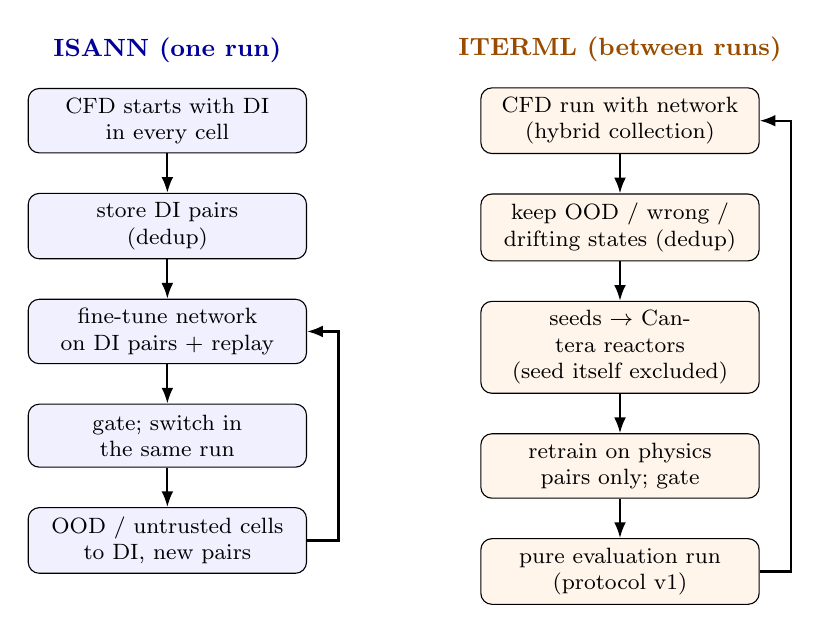
\begin{tikzpicture}[font=\footnotesize, node distance=5mm and 6mm,
  box/.style={draw, rounded corners, align=center, minimum height=8mm, text width=33mm},
  arr/.style={-{Latex[length=2mm]}, thick}]
\node[box, fill=blue!6] (i1) {CFD starts with DI\\in every cell};
\node[box, fill=blue!6, below=of i1] (i2) {store DI pairs\\(dedup)};
\node[box, fill=blue!6, below=of i2] (i3) {fine-tune network\\on DI pairs + replay};
\node[box, fill=blue!6, below=of i3] (i4) {gate; switch in\\the same run};
\node[box, fill=blue!6, below=of i4] (i5) {OOD / untrusted cells\\to DI, new pairs};
\draw[arr] (i1)--(i2); \draw[arr] (i2)--(i3); \draw[arr] (i3)--(i4); \draw[arr] (i4)--(i5);
\draw[arr] (i5.east) -- ++(4mm,0) |- (i3.east);
\node[above=2mm of i1, font=\small\bfseries, text=blue!60!black] {ISANN (one run)};
\node[box, fill=orange!8, right=22mm of i1] (t1) {CFD run with network\\(hybrid collection)};
\node[box, fill=orange!8, below=of t1] (t2) {keep OOD / wrong /\\drifting states (dedup)};
\node[box, fill=orange!8, below=of t2] (t3) {seeds $\rightarrow$ Cantera reactors\\(seed itself excluded)};
\node[box, fill=orange!8, below=of t3] (t4) {retrain on physics\\pairs only; gate};
\node[box, fill=orange!8, below=of t4] (t5) {pure evaluation run\\(protocol v1)};
\draw[arr] (t1)--(t2); \draw[arr] (t2)--(t3); \draw[arr] (t3)--(t4); \draw[arr] (t4)--(t5);
\draw[arr] (t5.east) -- ++(4mm,0) |- (t1.east);
\node[above=2mm of t1, font=\small\bfseries, text=orange!60!black] {ITERML (between runs)};
\end{tikzpicture}
\caption{The two loops. In ISANN the CFD's DI results are the training labels and the network changes
during the run. In ITERML the CFD only provides starting points for physics-based exploration; training
happens between runs and on Cantera data alone.}
\label{fig:loops}
\end{figure}

Table~\ref{tab:design} summarises the differences.

\begin{table}[t]
\centering
\caption{Design differences between the two schemes.}
\label{tab:design}
\small
\resizebox{\textwidth}{!}{%
\begin{tabular}{lll}
\toprule
 & ISANN & ITERML \\
\midrule
Role of the CFD states & training pairs (state, $\Delta t$, DI result) & seeds: where to explore \\
Origin of the training labels & DI of the running CFD & Cantera reactors started from seeds \\
CFD state in the training set & yes & never (excluded, with a \num{1e-8} margin) \\
When the network changes & during the run (control file) & between runs \\
DI needed in the production run & yes (DI phase, fallback) & no (pure mode) \\
Error detection & OOD + shadow checks & OOD + shadow checks + multi-step sentinel \\
Parent network & ood7 & ood8 \\
Model label & adapted to this simulation & a priori + seeded exploration \\
\bottomrule
\end{tabular}}
\end{table}

\subsection{Fairness of the comparison}
\label{sec:fair}
The comparison is not perfectly controlled, and the differences are stated here rather than hidden in the
results. (i) The parents differ (ood7 for ISANN, ood8 for ITERML); ood8 has a better a priori coverage of
the flame but, like ood7, ignites the fuel jet early in pure mode. (ii) ISANN's headline run is hybrid, by
design; the fair counterpart of an ITERML evaluation is therefore the final ISANN network (v6) run alone in
pure mode under the same protocol, which we report as the main ISANN result. (iii) The pure v6 run used
two ranks and the ITERML evaluation four, so costs per step are not directly comparable. (iv) Each
network was trained once; the spread between training seeds on the offline benchmark is about 15~K at
10~ms, comparable with some of the differences reported.
\todo{Repeat ISANN from ood8, or ITERML from ood7, to remove (i); retrain both finals with three seeds.}

%% ===============================================================================================
\section{Results}
\label{sec:results}

\subsection{How much information each scheme takes from the CFD}
\label{sec:data}
ISANN's first run kept its DI phase to 11.2~ms, accepted six networks (v1--v6, at 11.2, 15.4, 20.0, 23.7,
28.7 and 36.2~ms) in twelve rounds, and trained on about \num{35000} deduplicated DI pairs of the run,
replayed with three a priori pairs each; about a quarter of every training batch was therefore CFD data.

ITERML's first collection run (iteration-0 network ood8) stopped at 9.2~ms (458 steps) with \num{16033}
stored states. Of these, \num{13732} were seed candidates and \num{7891} remained after the radius of
novelty (Table~\ref{tab:seeds}); 70\% are lean ($Z<Z_\mathrm{st}=0.055$). The 2372 shadow checks of the
run failed in 4.3\% of the cases, and one of 31 sentinels drifted. The seeded exploration produced
\num{120719} pairs (the 35\% cap) in 7~min, and none of them is a CFD state. The second collection run,
with the iteration-1 network, a sentinel four times as dense and a wider ignition rule (fuel and O$_2$ at
800--1700~K), stored about \num{15200} states, which gave \num{2912} seeds after deduplication against
iteration 1, 173 of them ignition seeds. \pending{seeded pairs per regime, training time, gate result.}

\begin{table}[t]
\centering
\caption{ITERML seeds of iteration 1, by seeded regime and by the reason they were caught. Weight: CFD
states merged into the seeds of the regime.}
\label{tab:seeds}
\small
\begin{tabular}{lrrrrr}
\toprule
Regime & Seeds & Weight & $T$ median [K] & $Z$ median & $\psi$ median \\
\midrule
10 PaSR        & 2401 & 3791 & 1029 & 0.025 & 0.16 \\
11 relaxation  & 4924 & 9075 & 1638 & 0.047 & 0.12 \\
12 ignition    & 1    & 1    & 1508 & 0.129 & 0.04 \\
13 cooling     & 565  & 865  & 749  & 0.028 & 0.63 \\
\midrule
\multicolumn{6}{l}{Caught as: OOD 3104; untrusted bin + shadow error 2400; untrusted bin 2263;}\\
\multicolumn{6}{l}{shadow error 93; OOD + shadow error 30; sentinel drift 1.}\\
\bottomrule
\end{tabular}
\end{table}

The single ignition seed of iteration 1 is the main lesson of this stage: ignition errors build over many
steps in cells where every single step is inside the training data and passes a one-step shadow check,
so neither OOD flags nor shadow checks catch them, and the first sentinel was too sparse. ISANN does not
have this problem during its own run, because its DI phase integrates the ignition exactly; it shows it
when the trained network is reused from the start (Section~\ref{sec:ignition}).

\subsection{Established flame}
\label{sec:flame}
Figure~\ref{fig:flame} and Table~\ref{tab:main} show the errors against DI. In the established flame
(25--50~ms) all the adapted networks are within a few kelvin of DI, while the a priori ood1 network in
pure mode is 68.8~K off and drifts. The ISANN v6 network alone gives 2.1~K with a bias of $+0.8$~K and a
drift of $-0.5$~K per 10~ms; ITERML iteration 1 gives 3.3~K with a bias of $-1.5$~K. The ITERML error is
still falling at the end of the window (from 5.3~K at 25~ms to 1.7~K at 47.5--50~ms, a drift of $-1.6$~K
per 10~ms), so its 50~ms value equals that of v6. By zone, ITERML's largest errors are in the reactive
(5.5~K) and rich (7.4~K) zones, against 1.8 and 3.9~K for v6; the 95th percentile of the hot-cell error is
5~K against 2~K. The ISANN run itself, with DI fallback and changing networks, gives 2.0--3.4~K (mean
2.6~K); it is not lower than v6 alone because the network changed during the window. Both pure networks
reproduce the volume above 1500~K within 1\% and the position of the flame tip and base on the axis to
better than the 0.5~mm resolution of the analysis. The ITERML evaluation run had 0.9\% of the hot cells OOD
during the flame phase (none of them sent to DI), and its 4571 shadow checks had a median one-step
error of 0.027~K and a 5\% error of the temperature increment.

\pending{flame error, bias, drift, zone errors and OOD share of iteration 2; whether the 5~K target and the
2~K/10~ms drift target are met.}

\begin{figure}[t]
\centering
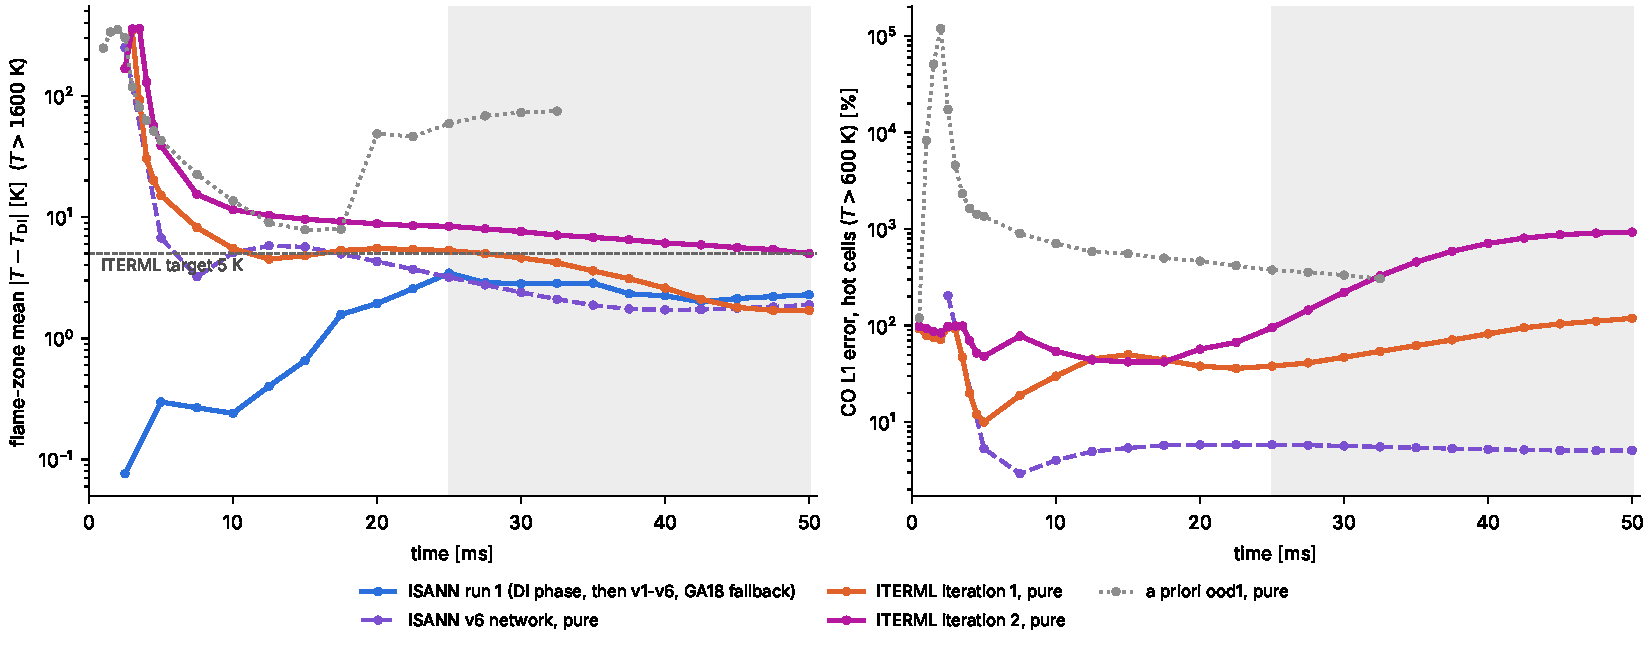
\includegraphics[width=\textwidth]{figs/fig_flame_error.pdf}
\caption{Left: mean temperature error in the flame zone ($T>1600$~K) against DI. Right: L1 error of CO in
hot cells ($T>600$~K). Shaded: the scored flame window. ISANN run~1 has the DI phase up to 11.2~ms, so its
early error is that of a restart; the pure runs use the network in every cell from the first step. The
pure v6 run was written every 2.5~ms only. ood1 pure was stopped at 32.5~ms.}
\label{fig:flame}
\end{figure}

\begin{table}[t]
\centering
\caption{Protocol v1 against GA18 DI. Pure: network in every cell, no DI fallback. Flame: mean
$|T-T_\mathrm{DI}|$ for $T>1600$~K over 25--50~ms. Totals: domain amount, model/DI, mean over 25--50~ms.
DI ignites at about 2.6~ms.}
\label{tab:main}
\small
\resizebox{\textwidth}{!}{%
\begin{tabular}{lccccc}
\toprule
 & ISANN run 1 & ISANN v6 & ITERML iter.~1 & ITERML iter.~2 & ood1 \\
 & (hybrid) & (pure) & (pure) & (pure) & (pure) \\
\midrule
Training data from the CFD             & DI pairs & DI pairs & none & none & none \\
Ignition time, model $-$ DI [ms]        & 0 (DI phase) & $-0.4$ & $+0.6$ & \pending{} & $-1.6$ \\
Worst flame bias at start-up [K]        & -- & $+251$ & $-345$ & \pending{} & $+351$ \\
Flame $|dT|$, 25--50 ms [K]             & 2.6 & 2.1 & 3.3 & \pending{} & 68.8$^a$ \\
Flame bias [K]                          & $-0.6$ & $+0.8$ & $-1.5$ & \pending{} & $-51^b$ \\
Drift [K per 10 ms]                     & -- & $-0.5$ & $-1.6$ & \pending{} & $+20^a$ \\
Flame $|dT|$ at 50 ms [K]               & 2.3 & 1.9 & 1.7 & \pending{} & -- \\
OH total, model/DI                      & -- & 0.55 & 1.05 & \pending{} & -- \\
CO total, model/DI                      & -- & 0.97 & 1.66 & \pending{} & -- \\
CH$_4$ total, model/DI                  & -- & 1.00 & 1.27 & \pending{} & -- \\
H total, model/DI                       & -- & 0.89 & 1.19 & \pending{} & -- \\
CO L1, hot cells                        & -- & 5\% & 75\% & \pending{} & 300--400\% \\
Heat release, model/DI                  & -- & 0.92$^c$ & 1.21 & \pending{} & -- \\
GA18 / OOD share, flame phase           & 0.14--0.5\% / $<$0.2\% & 0 / 0 & 0 / 0.9\% & \pending{} & 0 / -- \\
Cost [s per step]                       & 4.2 (2 ranks) & 2.85 (2 ranks) & 1.99 (4 ranks) & \pending{} & -- \\
\bottomrule
\multicolumn{6}{l}{\footnotesize $^a$ 25--32.5~ms, run stopped at 32.5~ms. $^b$ at 25~ms.
$^c$ flame zone only.}
\end{tabular}}
\end{table}

\subsection{Start-up and ignition}
\label{sec:ignition}
The start-up separates the two schemes most clearly (Fig.~\ref{fig:ignition}). Every a priori network of
this project ignites the fuel jet early in pure mode: ood1 by 1.6~ms, ood8 by about 1.5~ms (the
iteration-0 network of ITERML; $+348$~K at 2~ms in the ITERML test run). The ISANN network v6, adapted with
DI pairs that include the ignition, still ignites 0.4~ms early ($+251$~K in the first flame cells at
2.5~ms): its training pairs come from a DI phase in which the ignition happened once, and the
deduplication keeps one pair per region, so the few induction pairs weigh little. ITERML iteration 1
removed the early ignition but overshot: the jet ignites 0.6~ms late ($-345$~K at 3.0~ms), after which
the error decays to 15~K at 5~ms. The seeded relaxation and PaSR data (Table~\ref{tab:seeds}) slowed the
radical build-up in the induction zone, and the single ignition seed could not balance it. Iteration~2
was designed for exactly this: a four-times denser sentinel and an ignition rule that sends every seed
with fuel and oxygen at 800--1700~K to the ignition reactors, giving 173 ignition seeds.

\pending{ignition time of iteration 2, worst start-up bias, and whether the 0.3~ms target is met; add
the iteration-2 curve to Fig.~\ref{fig:ignition} (the script draws it automatically).}

\begin{figure}[t]
\centering
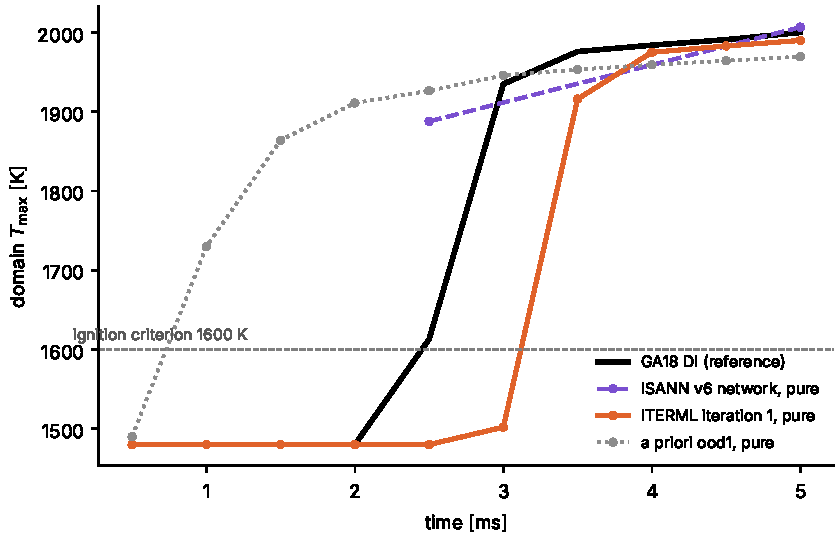
\includegraphics[width=0.7\textwidth]{figs/fig_ignition.pdf}
\caption{Maximum temperature in the domain during start-up, pure runs, against DI. The dashed line is the
ignition criterion of the protocol. The pure v6 run has no snapshot before 2.5~ms.}
\label{fig:ignition}
\end{figure}

\subsection{Species and heat release}
\label{sec:species}
Away from temperature the ISANN network is clearly better. With v6, total CO is within 3\% of DI and its
hot-cell L1 error is 5\%; total OH is 0.55 of DI. With ITERML iteration 1, total OH is right
(1.05), but CO, CH$_4$ and H are 27--66\% too high and the CO error grows steadily in the flame window, from
38\% at 25~ms to 119\% at 50~ms (Fig.~\ref{fig:flame}, right), together with the heat release evaluated on
the states (from 1.04 to 1.43 times DI, Fig.~\ref{fig:hrr}). The error is not in the flame itself, where
the CO L1 error is 2\%, but in the hot gas between 600 and 1600~K, i.e.\ in the slow CO oxidation of the
burnt gas recirculating under the pot. That region is covered by the cooling and relaxation seeds, but
their reactors run for at most 20~ms, while the gas stays under the pot for longer. ISANN does not have
this problem because its DI pairs are taken in that very gas.

\pending{CO, OH, H and heat-release ratios of iteration 2; whether the CO growth persists.}

\begin{figure}[t]
\centering
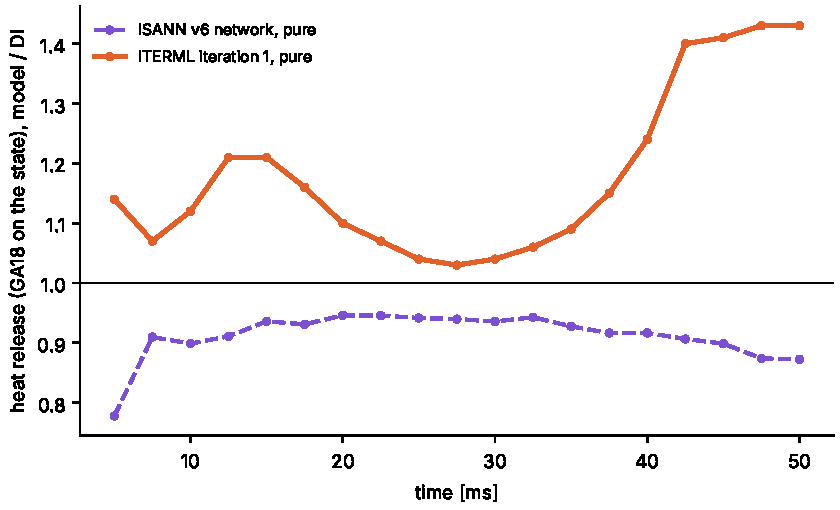
\includegraphics[width=0.7\textwidth]{figs/fig_hrr.pdf}
\caption{Heat-release rate obtained by evaluating GA18 on the model's state, over the domain, relative to
DI, pure runs.}
\label{fig:hrr}
\end{figure}

\subsection{Generality away from the burner}
\label{sec:offline}
On the offline benchmark the two schemes behave differently. The ISANN v6 network ranked first among the
networks of the project on 440 canonical states (score 1.75 against 2.38 for its parent ood7 and 2.88 for
ood1): fine-tuning on the flame's DI pairs with replay did not cost generality. The ITERML iteration-1
network lost some accuracy on the 218-state set against its parent ood8 (mean $|dT|$ at 10~ms 31.8 against
28.2~K, at 50~ms 59 against 51~K; equilibrium fixed point 42 against 27~K), within the seed-spread
tolerance of the gate. The loss is concentrated in vitiated states (85 against 53~K at 10~ms), while
partially burnt and cooled states improved (69 against 103~K at 10~ms, and 11 against 34~K at 50~ms). A
35\% share of seeded data drawn from one burner's burnt gas thus displaces part of the a priori
coverage, even though no CFD state is in it. \todo{Run both final networks on the same 440-state set with
three training seeds each; the two sets above are not the same.}
\pending{offline benchmark of iteration 2 against iteration 1 and ood8.}

\subsection{Cost}
\label{sec:cost}
ISANN pays for its labels during the production run: the DI phase cost 7.9~s per step on two ranks and the
network phase 4.2~s, and the first 50~ms took 3.5~h; once trained, v6 alone ran at 2.85~s per step on two
ranks. ITERML pays between runs: iteration 1 took about 2.5~h of wall time on four cores (collection run
18~min, seeds and seeded exploration 7~min, warm-start training 32~min, gate 2~min, pure evaluation
to 50~ms the rest), and the pure network ran at 1.99~s per step on four ranks. The production run of an
ITERML network needs no DI at all, so it can run in a solver without a hybrid mode; a reused ISANN
network (Section~\ref{sec:ignition}) has the same property but carries CFD data in its training set.
\todo{Same-rank timing of v6 and ITERML networks; DI cost on four ranks.}

%% ===============================================================================================
\section{Discussion}
\label{sec:discussion}

\paragraph{Labels or locations} Using the simulation's DI results as labels gives the most accurate
network for that simulation: v6 is the best network of the project on flame temperature, CO and heat
release. Using the simulation only to choose locations reaches the same flame temperature by 50~ms with
training data that remain a model of the mechanism, but it converges more slowly and depends on the
exploration reproducing the relevant states from a seed. Where the physics of the seeded reactor is
right (burnt-gas relaxation, PaSR mixing), one iteration is enough; where it is not (long-residence CO
oxidation, ignition from a handful of seeds), the error is visible in the next evaluation and points to
the regime that needs work, which is a diagnostic ISANN does not offer.

\paragraph{What each detector sees} Both schemes rely on OOD flags and one-step shadow checks, and both
miss multi-step errors inside the training data: ISANN's v6 network ignites early without a single OOD
cell or failed check, and ITERML's first collection caught one ignition state out of \num{16033}. The
multi-step sentinel of ITERML is the only element of either scheme that targets this error, and its
density matters.

\paragraph{Mirror-image ignition} The a priori and ISANN networks ignite early, ITERML's first network
late. The ignition delay of the jet is set by a few cells in the induction zone; a network that is
slightly too reactive there ignites early and one slightly too slow ignites late, and neither shows up
in the flame-zone error once the flame is established. The ignition time must therefore be scored
separately, as protocol v1 does, and should be part of the acceptance gate of both schemes.

\paragraph{When to use which} For repeated simulations of one configuration where DI can run in the
production solver, ISANN gives the best accuracy at the lowest effort. When the surrogate must run in a
solver without DI fallback, must be reported as a physics-based model, or will be transferred to other
conditions, ITERML keeps the training data clean and still uses the simulation to direct the effort.
\pending{revise this paragraph if iteration 2 closes the ignition and CO gaps.}

\paragraph{Limitations}
\begin{itemize}
\item One laminar 2D configuration, one mechanism and one fuel. \todo{second, turbulent case}
\item Different parent networks (ood7 vs ood8) and one training seed per network (Section~\ref{sec:fair}).
\item Only one complete ITERML iteration at the time of writing \pending{update}; the loop's stop
  criteria have not been reached yet.
\item The evaluation covers 0--50~ms of a transient; the steady state was tested with local time stepping
  for ISANN only (flame error 40--48~K against a DI solution that itself drifts by 100~K, with CO frozen in
  cold long-residence gas).
\item The circularity of ITERML: the seeds come from this burner, so the seeded data emphasise its
  states even though they are physics data; the a priori and ITERML networks are therefore reported side
  by side, and the offline benchmark measures the cost.
\item No comparison with ISAT on the same machine.
\end{itemize}

%% ===============================================================================================
\section{Conclusions}
\label{sec:conclusions}
Two ways of letting a reacting-flow simulation improve its chemistry surrogate were compared on a laminar
methane/air burner with an 18-species mechanism, under one evaluation protocol in pure mode:
\begin{enumerate}
\item learning from the run's DI pairs (ISANN) gave the most accurate network: 2.1~K mean flame error,
  total CO within 3\%, and first place on an offline benchmark of canonical states;
\item seeding physics-based exploration with the states where the network fails (ITERML) gave 3.3~K
  (1.7~K at 50~ms) after one iteration, with no CFD state in the training data, but too much CO and heat
  release in the recirculating hot gas and a small loss on the offline benchmark;
\item both schemes miss multi-step ignition errors with one-step checks; ISANN's network ignites the jet
  0.4~ms early and ITERML's first network 0.6~ms late \pending{iteration 2};
\item the information the simulation gives about \emph{where} the network fails is enough to reach a
  few-kelvin flame error without using the simulation's results as labels.
\end{enumerate}
\pending{final conclusion after iteration 2.}

\section*{Data and code availability}
\todo{Repository (chemmanifold-studio: openfoam/isann, openfoam/iterml, openfoam/protocol,
scripts/19\_iterml\_seeds.py, chemmanifold/seeded.py), model files and protocol reports.}

\section*{Acknowledgements}
\todo{}

\bibliographystyle{elsarticle-num}
\bibliography{refs}

\end{document}
